\begin{figure}[htbp]
    \centering
    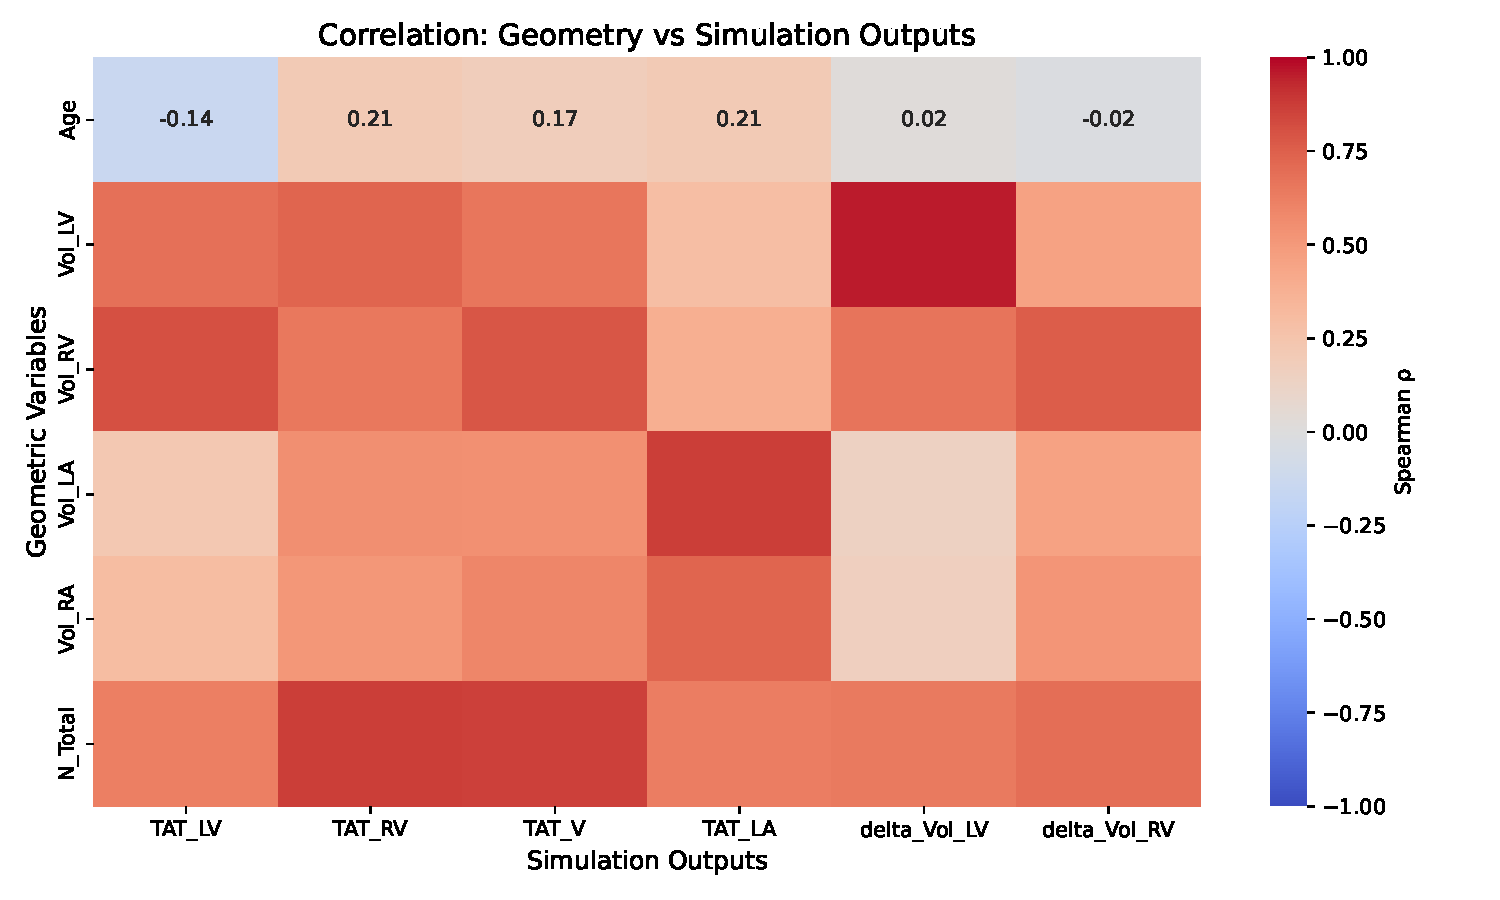
\includegraphics[width=\textwidth]{pics/sp2_correlation_heatmap.pdf}
    \caption{
        \textbf{Correlation matrix between geometric variables and simulation outputs.}
        Spearman correlation coefficients ($\rho$) shown for relationships between
        geometric metrics (chamber volumes, myocardial wall volume, age) and simulation
        outputs (activation times, volume changes). Strong positive correlations
        (red) indicate that geometric variables predict functional outcomes under
        standardised parameters. All correlations shown are statistically
        significant ($p < 0.05$).
}
    \label{fig:s3-correlation-heatmap}
\end{figure}
